\documentclass[11pt, aspectratio=169]{beamer}
\usepackage[utf8]{inputenc}
\usepackage{float}
\usepackage[english]{babel}
\usepackage{tikz-cd}
\usepackage{amsthm}
\usepackage{bbm}
\usepackage{enumitem}
\usepackage{tikz}
\usepackage{amsmath}
\usepackage{amsfonts}
\usepackage{amssymb}
\usepackage{mathtools}
\usepackage{graphicx}
\usepackage{rotating}
\usepackage{setspace}
\usepackage{color}
\usepackage{fancyhdr}
\usepackage{ragged2e}
\usepackage{appendix}
\usepackage{tabularx}
\usepackage{multirow}
\usepackage{booktabs}
\usepackage{xfrac}
\usepackage{xcolor}
\usepackage{pgfplots}
\usepackage{url}
\usepackage{emptypage}
\usepackage{wrapfig}
\usepackage{dsfont}
%\usepackage{makecell}
\usepackage{bm}
%\usepackage{csquotes}



\pgfplotsset{compat=1.18}



%Operators
\DeclareMathOperator{\CVar}{CVar}
\DeclareMathOperator{\Span}{Span}
\DeclareMathOperator{\fq}{q}
\DeclareMathOperator{\fb}{b}

%shortcuts
\newcommand{\nc}{\newcommand} 
\nc{\cH}{{\mathcal H}}
\nc{\cR}{{\mathcal R}}
\nc{\cA}{{\mathcal A}}
\nc{\cG}{{\mathcal G}}
\nc{\cC}{{\mathcal C}}
\nc{\cD}{{\mathcal D}}
\nc{\cO}{{\mathcal O}}
\nc{\cI}{{\mathcal I}}
\nc{\cB}{{\mathcal B}}
\nc{\cY}{{\mathcal Y}}
\nc{\cK}{{\mathcal K}} 
\nc{\cX}{{\mathcal X}}
\nc{\cS}{{\mathcal S}}
\nc{\cE}{{\mathcal E}}
\nc{\cF}{{\mathcal F}}
\nc{\cZ}{{\mathcal Z}}
\nc{\cQ}{{\mathcal Q}}
\nc{\cN}{{\mathcal N}}
\nc{\cP}{{\mathcal P}}
\nc{\cL}{{\mathcal L}}
\nc{\cM}{{\mathcal M}}
\nc{\cT}{{\mathcal T}}
\nc{\cW}{{\mathcal W}}
\nc{\cU}{{\mathcal U}}
\nc{\cJ}{{\mathcal J}}
\nc{\cV}{{\mathcal V}}
\nc{\bH}{{\mathbb H}}
\nc{\bA}{{\mathbb A}}
\nc{\bG}{{\mathbb G}}
\nc{\bC}{{\mathbb C}}
\nc{\bO}{{\mathbb O}}
\nc{\bI}{{\mathbb I}}
\nc{\bB}{{\mathbb B}}
\nc{\bY}{{\mathbb Y}}
\nc{\bK}{{\mathbb K}} 
\nc{\bX}{{\mathbb X}}
\nc{\bS}{{\mathbb S}}
\nc{\bE}{{\mathbb E}}
\nc{\bF}{{\mathbb F}}
\nc{\bZ}{{\mathbb Z}}
\nc{\bQ}{{\mathbb Q}}
\nc{\bN}{{\mathbb N}}
\nc{\bP}{{\mathbb P}}
\nc{\bL}{{\mathbb L}}
\nc{\bM}{{\mathbb M}}
\nc{\bT}{{\mathbb T}}
\nc{\bW}{{\mathbb W}}
\nc{\bU}{{\mathbb U}}
\nc{\bD}{{\mathbb D}}
\nc{\bJ}{{\mathbb J}}
\nc{\bV}{{\mathbb V}}
\nc{\bR}{{\mathbb R}}

\nc{\boB}{{\mathbf{B}}}
\nc{\boL}{{\mathbf{L}}}
\nc{\boG}{{\mathbf{G}}}


\nc{\tV}{{\Tilde{{V}}}}
\nc{\tI}{{\Tilde{{I}}}}
\nc{\tY}{{\Tilde{{Y}}}}
\nc{\tS}{{\Tilde{{S}}}}

\nc{\fr}{{\rightarrow}}
\nc{\co}{{\nabla}}

\newcommand{\la}{\; \longrightarrow \;}
\nc{\cu}{{\barline{\nabla}}}


\usepackage[
backend=biber,
style=alphabetic,
sorting=nty
, maxbibnames=99]{biblatex}

\addbibresource{sample.bib}




\usepackage{ragged2e} % giustifica
\justifying
\setbeamertemplate{caption}{\insertcaption}
\setbeamercovered{invisible}
%\setbeamertemplate{footline}[frame number]
\usepackage{tikz}
\usetikzlibrary{arrows,%
                shapes,positioning}
                
                \definecolor{blendedblue}{rgb}{0.2,0.2,0.7}
        
\usetikzlibrary{%
                petri,%
                topaths}%
%\usepackage{tikz-berge}


\usepackage{ifpdf} 
\ifpdf% 
        \usepackage{pdftricks} 

        \begin{psinputs} 
            \usepackage{pstricks} 
            \usepackage{pstricks-add} 
            \usepackage{pst-plot} 
            \usepackage{pst-text,pst-node,pst-tree} 
        \end{psinputs} 
\else 
        \usepackage{pstricks} 
        \usepackage{pstricks-add} 
        \usepackage{pst-plot} 
        \usepackage{pst-text,pst-node,pst-tree} 

\fi 

\usepackage{pstricks}

\makeatletter
\setbeamertemplate{footline}
{
  \leavevmode%
  \hbox{%
  \begin{beamercolorbox}[wd=.333333\paperwidth,ht=2.25ex,dp=1ex,left]{author in head/foot}%
    \usebeamerfont{author in head/foot}\hspace*{2ex}\insertauthor
  \end{beamercolorbox}%
  \begin{beamercolorbox}[wd=.333333\paperwidth,ht=2.25ex,dp=1ex,center]{title in head/foot}%
    \usebeamerfont{title in head/foot}\insertsubsection
  \end{beamercolorbox}%
  \begin{beamercolorbox}[wd=.333333\paperwidth,ht=2.25ex,dp=1ex,right]{date in head/foot}%
    \usebeamerfont{date in head/foot}\insertshortdate{}\hspace*{2em}
    \insertframenumber{} / \inserttotalframenumber\hspace*{2ex} 
  \end{beamercolorbox}}%
  \vskip0pt%
}
\makeatother
\setbeamertemplate{navigation symbols}{}

\usepackage{color}
\definecolor{deepblue}{rgb}{0.3,0.3,0.9}
\definecolor{deepred}{rgb}{0.6,0,0}
\definecolor{deepgreen}{rgb}{0,0.5,0}

\setlist[itemize]{label=\textcolor{deepblue}{\rule[0.5ex]{1ex}{1ex}}}
\usepackage{listings}

\definecolor{codegreen}{rgb}{0,0.6,0}
\definecolor{codegray}{rgb}{0.5,0.5,0.5}
\definecolor{codepurple}{rgb}{0.58,0,0.82}
\definecolor{backcolour}{rgb}{0.95,0.95,0.92}

\lstdefinestyle{mystyle}{
    backgroundcolor=\color{backcolour},   
    commentstyle=\color{codegreen},
    keywordstyle=\color{magenta},
    numberstyle=\tiny\color{codegray},
    stringstyle=\color{codepurple},
    basicstyle=\ttfamily\footnotesize,
    breakatwhitespace=false,         
    breaklines=true,                 
    captionpos=b,                    
    keepspaces=true,                 
    numbers=left,                    
    numbersep=5pt,                  
    showspaces=false,                
    showstringspaces=false,
    showtabs=false,                  
    tabsize=2
}

\lstset{style=mystyle}


\newtheorem{prop}[theorem]{Proposition}
\newtheorem{defi}[theorem]{Definition}
\newtheorem{oss}[theorem]{Observation}
\newtheorem{theo}[theorem]{Theorem}
\newtheorem{cor}[theorem]{Corollary}
\newtheorem{assumption}[theorem]{Assumption}
\renewcommand*{\bibfont}{\footnotesize}




\title{A Parallelization Algorithm for Adequacy Assessment of the Electrical Grid}
\author{Gabor Riccardi}
\date{\today}
\institute{Università di Pavia}

\begin{document}

\begin{frame}[plain]
  \begin{minipage}{0.3\textwidth}
    \centering
    
\includegraphics[width=.6\linewidth]{unipv.png}\\[\baselineskip] % Adjust space as needed
    
\includegraphics[width=.8\linewidth]{EC-JRC-logo.png}
  \end{minipage}%
  \begin{minipage}{0.05\textwidth}
    \tikz[remember picture, overlay] \draw[yellow, thick] (0,0) -- (0,-\textheight);
  \end{minipage}%
  \begin{minipage}{0.65\textwidth}
    \maketitle
    \centering
    
\includegraphics[width=.6\linewidth]{AIROY.png}
  \end{minipage}    
\end{frame}


\section{Brief Overview of Power Grid Optimization Problems}
\begin{frame}{Power Grid Optimization problems 1}
  
    \begin{figure}
        \centering
        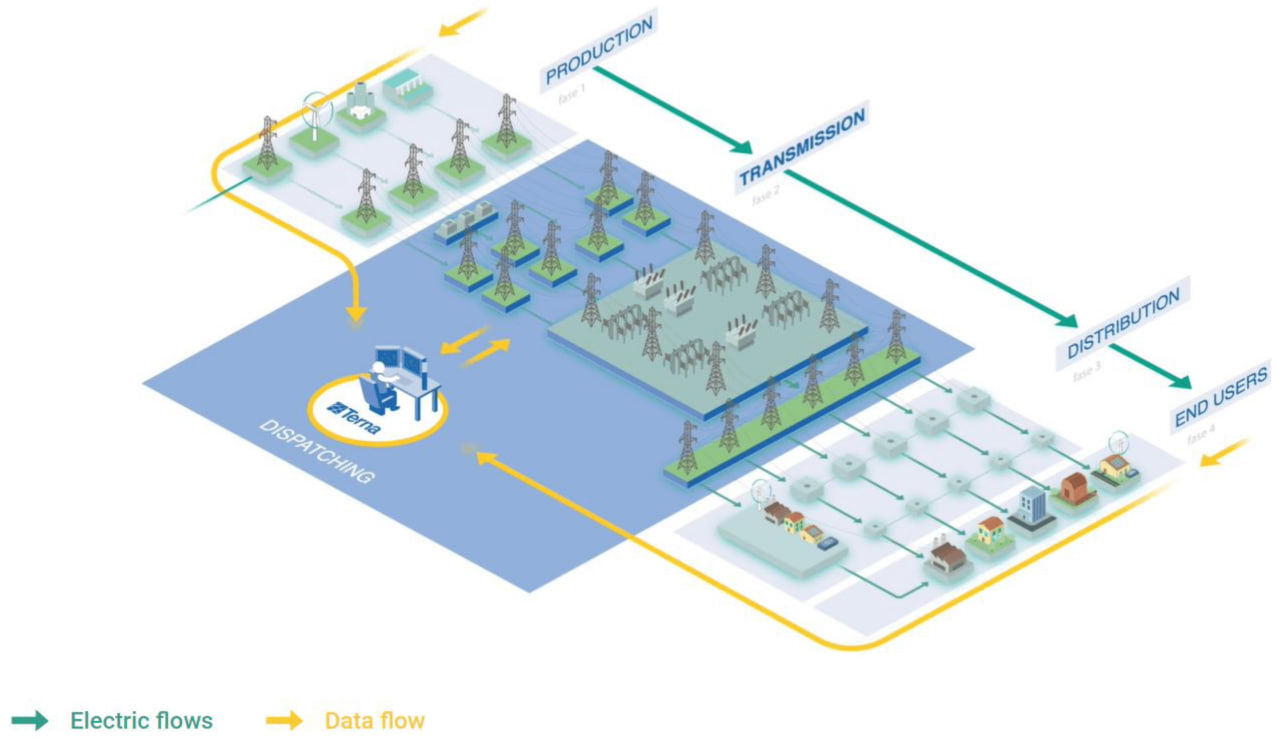
\includegraphics[width=0.8\textwidth]{photo_2023-09-26_14-27-16.jpg}

        \label{fig:enter-label}
    \end{figure}
\end{frame}



\begin{frame}{Power Grid Optimization: From Simple to Exact Models}
    \begin{itemize}
      \item Optimal Power Flow (OPF) \hfill \textcolor{gray}{\cite{MathProgForm}}
        \begin{itemize}
          \item AC OPF: exact physical model 
          \item Security-Constrained OPF (SCOPF) -- Includes contingencies to guarantee system security under failures.
          \item DC OPF and other linearized models \hfill \textcolor{gray}{\cite{LinRelBien} }
          \item other relaxations. 
        \end{itemize}
       
      \item Unit Commitment -- Determines on/off status of power units, ignoring grid constraints.
      \item Economic Dispatch (ED) -- Minimizes generation cost, ignoring grid constraints.  
    \end{itemize}
    % Blue arrow on the side of the text
    \begin{tikzpicture}[overlay, remember picture]
      \node at ([shift={(0.9,-1)}]current page.north west) (end0) {}; % Adjust for positioning
      \node at ([shift={(0.9,3)}]current page.south west) (start0) {}; % Adjust for positioning
      \draw[->, thick, blue] (start0) -- (end0) node[midway, fill=white, rotate=90] {Time / Exactness};
  
      \node at ([shift={(0.3,-1)}]current page.north west) (start1) {}; % Corrected position and syntax
      \node at ([shift={(0.3,3)}]current page.south west) (end1) {}; % Corrected position and syntax
      \draw[->, thick, yellow] (start1) -- (end1) node[midway, fill=white, rotate=90] {Stochasticity}; % Corrected spelling and syntax
  \end{tikzpicture}
  
    \vfill
    \textbf{Adequacy Assessment Model:} Based on Economic Dispatch models with added flow balance at bus nodes and various scenarios.
\end{frame}

\begin{frame}{Economic Dispatch (ED) model\textcolor{red}{*}}
  For a fixed scenarios \(w\) let \: \( y_w = (p_w,f_w,ls_w )'\) be the vector containing the power genaration, power flows and line shedding variables.
  \begin{align}
    \min_{y} \; & q'y_w \\
    s.t. \; & p_{n,g,t,w} \leq x_{n,g} \\
         & L^{\text{min}}_{n, l} \leq f_{n,l,t,w} \leq L^{\text{max}}_{n, l} \\
         & v_{n,t,w} = v_{n,t-1,w} + BCE \cdot bc_{n,t,w} - BDE \cdot bd_{n,t,w} + A_{n,t,w}\\
         & (v_{n,t,w}, bc_{n,t,w}, bd_{n,t,w}) \leq (BV, BC, BD) \\
         & p_{n,g,t,w} + bd_{n,t,w} + \sum_{l \in \cL(n)}f_{n,l,t,w} + ls_{n,t,w} + \mathcal{PV}_{n,t,w} + \cW_{n,t,w} = \\
         & =  \cD_{n,t,w} + ps_{nt.w} + bc_{n,t,w} 
  \end{align}
Where  \(w = (\mathcal{PV}, \mathcal{W}, \mathcal{D})\) represents the scenario realization of solar power, wind power and loads
\end{frame}

\begin{frame}{Stochastic Capacity Expansion Problem (CEP)}
  Let \(\cV(x,w)\) be the solution to (ED) in function of the expanded capacities \(x\) and the scenario \(w\).
  We formulate the Stochastic Capacity Expansion Problem as a two-stage stochastic program.
  \begin{itemize} 
    \item The first stage determines the capacity expansion \(x_{n,g}\) for each generator \(g \in \cG \)
    \item The second stage solves the (ED).
  \end{itemize}  
  \begin{align*}
    \label{CEP-A}
    \min_{x} \;&c'x + \bE_w\left[\cV(x,w)\right] \\  \tag{CEP}
    s.t. \; & 0 \leq x_{n,g} \leq X_{n,g} 
  \end{align*}
 
\end{frame}

\section{Models and sub-Models}

\begin{frame}{Literature}
  \begin{itemize}
    \item Traditional stochastic capacity expansion methods, such as the L-shaped method, may perform poorly as the number of expansion possibilities increases.
    \item A decomposition algorithm based on subgradient approximations was introduced by Daniel A'vila et al in \cite{DecompAlg}
    \item Building upon this work, we propose another subgradient approximation algorithm to enhance the decomposition approach.
    \item We take advantage of the time steps' general independence, except for the constraints related to batteries and storage, which rely on adjacent time steps.
    \item Our approximation is refined throught iterations to ensure convergence within a finite number of steps.
  \end{itemize}
\end{frame}

\begin{frame}{Model description 1}
  \begin{itemize}
    \item We divide the time horizon into \(K\) intervals, \(\{t_{0} = 0 \coloneqq 1,\ldots, t_{1}\},\{t_2,\ldots,t_3\},\ldots,\{t_{K-1},\ldots,t_K \coloneqq T\}\)
    \item If we fix a priori the storage values adding the constraints \( v_{t_{k}} = \bar v_{t_{k}}\) to (ED) we obtain a solution \(V(x,\{v_{t_{k}}\}_k, w)\) also dependent on these intermediary storage values.
    \item Then considering the (ED) problems restricted to each interval with fixed initial and final storage values and with optimal value \(V_{k}(x,v_{t_{k}},v_{t_{k+1},w})\).
  \end{itemize}
  
  \begin{oss}
    \begin{equation}\label{Divided ED eq}
      V(x,w) = \min_{\{v_{t_k}\}_{k=1}^K}\sum_{k=0}^{K-1}V_{k}(x,v_{t_{k}},v_{t_k+1},w)
    \end{equation}
  \end{oss}

\end{frame}

\begin{frame}{Model description 2}
Since each function \(V_k\) is peacewise linear convex in \(x,v_{t_K},v_{t_{K+1}}\), given a collection of supporting hyperplanes \(\{\pi^w_{i,k}(x,v_{t_k},v_{t_{k+1}})\}\) of each \(V_k\) an approximation of \eqref{Divided ED eq} is given by:

\begin{align}
  \hat{V}(x,w) = \min_{\{v_{t_k}\}_{k=1}^K} & \sum_{k=0}^K \theta_{k}^w \\
                \text{s.t.} \quad & \theta_k^w \geq \pi_{i,k}^w(x,v_{t_k,t_{k+1}}) \quad \forall i,k
\end{align}

\end{frame}
\begin{frame}{Model description 3}
Thus by substituting \(\cV\) with \( \hat{\cV} \) in (CEP) we obtain the following relaxation:
\begin{align*}
  \label{CEP-R}
  \min_{x} \;&c'x + \bE_w\left[\hat{\cV}(x,w)\right] \\  \tag{CEP-R}
  s.t. \; & 0 \leq x_{n,g} \leq X_{n,g} 
\end{align*}
  Since calculating \( \hat{\cV} \) is straightforward, solving (CEP-R) can be done efficiently with L-shaped or subgradient schemes.
\end{frame}  

\section{Decomposition Algorithm}

\begin{frame}{Algorithm description}
  INPUT: Provide a lower bound for \(\theta_k^{\omega}\) for \(k=1,\ldots,K\) and \( \omega \in \Omega \) and a trial action \(\hat x^0\)

  \begin{tabular}{@{}p{0.95\textwidth}}
    1. Warm-Start: Calculate initial approximation for \(\mathcal{V}\) for all \(w \in \Omega\) around \(\hat{x}^0\). \\
    2. For \(i = 1,\ldots,N\): \\
    \quad 2.1. For \(w \in \Omega \) (in parallel): \\
    \quad\quad\quad 2.1.1. Solve the (ED) approximation problem \(\hat{\mathcal{V}}(\hat{x}^{(i)},\omega)\) and obtain 
    \\ \quad\quad\quad\quad  intermediate storage values \(\hat{v}^i_k\) for \( k=1,\ldots,K\). \\
    \quad\quad\quad 2.1.2. Solve (ED) (in parallel) for each time step \(k = 0,\ldots,K-1\),
    \\ \quad\quad\quad\quad\(V_k(\hat{x}^i,\hat{v}^i_k, \hat{v}^i_{k+1},\omega)\). \\
    \quad\quad\quad 2.1.3. Using dual multipliers, compute a supporting hyperplane for \(V_k\) around 
    \\ \quad\quad\quad\quad\(\hat{x}^i, \hat{v}^i_k, \hat{v}^i_{k+1}\) for \(k=0,\ldots,K-1\). \\
    \quad\quad\quad 2.1.4. Add the supporting hyperplanes to the approximation problem (CEPR)
    \\ \quad\quad\quad\quad  \(\hat{\mathcal{V}}(\hat{x}^{(i)},\omega)\). \\

  \end{tabular}
\end{frame}

  
\section{Convergence results}
\begin{frame}{Convergence results 2}
  \begin{itemize}
    \item  Since (CEP-R) is a relaxation of (CEP), an optimal solution \(\hat x^i \) of (CEP-R) is also optimal for (CEP) iff it's (CEP)-feasible 
    \item Since the first stage constraints of (CEP-R) and (CEP) are the same this is true whenever, \(\hat x^i\) is feasible for the second stage problems
    \item This is true whenever  \(\cV(\hat x^i,w) = \hat{\cV}(\hat x^i,w) < + \infty \) for all \(\omega \in \Omega \) 
  \end{itemize}

  
  \textbf{Remark 1:} It is sufficient to prove the after a finite number of steps \((i)\) of the algorithm we have \(\hat{\cV}(\hat x^i,\omega) = \cV(\hat x^i,\omega) \) for all \( \omega \in \Omega \)
  



\end{frame}

\begin{frame}{Convergence results 3}
\begin{oss}
  Let \( \hat{\cV}_k(x,v_{t_k},v_{t_{k+1}},w) = \max_i \pi_{i,k}^w(x,v_{t_k},v_{t_{k+1}})\) be the current supporting hyperplane approximation of \(\cV_k\)
  Let \( \omega \in \Omega \) and \(k \in \{0,\ldots,K-1\}\). If after step (2.1.3) no new cuts are added then \(\hat{\cV}_k(x, v_{k},v_{k+1}) = \cV_k(x, v_{k},v_{k+1}). \) \\
  
\end{oss}
\begin{proof}
  
  Let \(\bar c_k^w(x,v_{t_k}) \coloneqq p'(x-\hat x^i, v_{t_k}-\hat v_{t_k}) + V_k(\hat x^i,\hat v_{t_k})\) be the new cut found after the \(i\)-th iteration. \\
  Since \(\bar c\) is not a new cut we have \( \bar c(x,v_{t_k}) \leq \hat{\cV}(x,v_{t_k})\).
  \\ Since \(\cV_k \geq \pi_{i,k}^w \), \(\cV_k \geq \hat{\cV}_k \). \\
  We have thus \[\cV_k(\hat x,\hat v_{t_k}) \geq \hat \cV_k(\hat x,\hat v_{t_k}) \geq \bar c (\hat x,hat v_{t_k}) = \cV(\hat x,\hat v_{t_k})\] which concludes the proof.
\end{proof}
\end{frame}

\begin{frame}{Convergence results 4}
  \begin{prop}
    After a finite number of iterations no new cuts are found for \(V_k\)
  \end{prop}
  \begin{proof}
    \begin{align}
      &\#\{p \mid p \text{ is a normal vector of a supporting hyperplane of } \mathcal{V}_k\} \leq \nonumber \\
      &\#\{\text{dual solutions } p=q'B^{-1} \text{ of (ED) for varying } x, v_{t_k}, v_{t_{k+1}}\} \leq \nonumber \\
      &\#\{\text{basis matrices of (ED)}\} < \infty 
    \end{align}
     After a finite number of steps we'll have a new cut \(\bar c (x,v)= p'(x,v) + b\) 
    with the same normal vector \(p\) as a previous cut \(\pi(x,v) = p'(x,v) + \bar b\). Since both are supporting hyperplanes it follows that \( b = \bar b\).
  \end{proof}
\end{frame}
\begin{frame}{Convergence results 5}
  In conclusion, we have \(\hat{\cV}_k(\hat x^i, v_{t_k},v_{t_{k+1}},\omega) = \cV_k(\hat x^i, v_{t_k},v_{t_{k+1}},\omega)\) for all \(\omega,k\).
   And from the definition of \(\hat \cV\) follows that \( \hat \cV(\hat x^i,w) = \cV(\hat x^i,w) \). 
   From Remark 1, it follows:
  \begin{prop}
    The algorithm converges after a finite number of iterations.
  \end{prop}
\end{frame}

\begin{frame}{Pypsa}
  Implementation coming soon in the PyPsa environment...

  \vspace{1cm}

  Thank you for your attention.
\end{frame} 
\section{Bibliography}
\begin{frame}{}
Some references:\\[2em]
\begin{footnotesize}
\printbibliography[
%heading=bibintoc,
title={Bibliography}]
\end{footnotesize}
\end{frame}

\begin{frame}[noframenumbering]{}
  further explanation
\end{frame}

\end{document}








